\documentclass[11pt,a4paper]{article}
\usepackage[T1]{fontenc}  
\usepackage[francais]{babel}
\usepackage[utf8]{inputenc}
\usepackage{pb-diagram} %                              pour construire des diagrammes commutatifs

%\usepackage{fancyhdr}
\pagestyle{plain}%                                             entête et pied de page
%\pagenumbering{arabic}%

%
\usepackage[vmargin=5cm]{geometry}%           marges en haut et en bas.

\setlength{\parskip}{5pt}%                                espace entre les paragraphes
%%x
%\setlength{\marginparwidth}{0.5cm}%
%\setlength{\hoffset}{-1in}%
%\setlength{\voffset}{-1in}%
%%\setlength{\evensidemargin}{1cm}%
%%\setlength{\oddsidemargin}{2cm}%
%\setlength{\textwidth}{17cm}%
%\setlength{\marginparsep}{0.1cm}%
%\setlength{\marginparwidth}{1.7cm}%
%\setlength{\topmargin}{1cm}%
%\setlength{\headheight}{1cm}%
%\setlength{\headsep}{1cm}%
%\setlength{\textheight}{24.0cm}%
%%
%\setlength{\oddsidemargin}{1.5cm}%
%\setlength{\evensidemargin}{1.5cm}%
%
\setlength{\parindent}{12pt}%                             indentation des paragraphes
%
\usepackage{color}%
\usepackage{mdwlist}%                                      pour liste
\usepackage{graphicx}%                                    insérer une image
%\usepackage{float}%                                           positionner des figures
\usepackage{here}
\usepackage{makeidx}%         				    pour faire index
\setcounter{secnumdepth}{3}%                      ??  numéroter les subsubsections
%
\usepackage{amsmath}%
\usepackage{amssymb}%
\usepackage{amsthm}%
\usepackage{amsfonts}%
\usepackage{mathrsfs}%
%\usepackage{bbm}%                                              lettres ensembles (N, Z, Q, R)
\usepackage[all,cmtip]{xy}%
%\xyoption{all}
\usepackage{rotate}%					       pivoter des objets
%\usepackage{yfonts}%                                            écritures gothiques, etc
%\usepackage{eurosans}
%\usepackage{mathabx}
%
\usepackage{graphicx}
\usepackage{caption}
\usepackage{eurosym}
%
\usepackage{array}% 
\usepackage{multirow}
%\usepackage[retainorgcmds]{IEEEtrantools}         					tableaux
%
\usepackage{natbib}


\usepackage{hyperref}

\usepackage{cleveref}

 
% fourier soit stmaryrd 
%\usepackage{fourier}
%Commandes d'environnement de théorèmes.
\newtheorem{Prop}{Proposition}[section]%
\newtheorem{Theo}[Prop]{Théorème}%                   la numérotation suit celle de 
\newtheorem{Def}[Prop]{Définition}%                      l'environnement "prop"
\newtheorem{Cor}[Prop]{Corollaire}%
\newtheorem{Lem}[Prop]{Lemme}%
\newtheorem{Conj}[Prop]{Conjecture}%
\newtheorem{Hyp}[Prop]{Hypothèse}%
\newtheorem{Question}[Prop]{Question}%
\newtheorem{Rq}[Prop]{Remarque}%
\newtheorem{Term}[Prop]{Terminologie}%
\newtheorem{Ex}[Prop]{Exemple}%
\newtheorem{Rap}[Prop]{Rappels}%
\newtheorem{PropDef}[Prop]{Proposition et définition}%
%
%[section]
%Lettres bb
\newcommand{\A}{\mathbb A}%
\newcommand{\C}{\mathbb C}%
\newcommand{\D}{\mathbb D}%
\newcommand{\E}{\mathbb E}%
\newcommand{\fp}{\mathbb F_{p}}%
\newcommand{\Fp}{\mathbb F}%
\newcommand{\G}{\mathbf G}%
\newcommand{\Gm}{\mathbb G}
\newcommand{\Hbb}{\mathbb H}
\newcommand{\N}{\mathbb N}%
\newcommand{\Pbb}{\mathbb P}%
\newcommand{\Q}{\mathbb Q}%
\newcommand{\qp}{\mathbb Q_{p}}%
\newcommand{\R}{\mathbb R}%
\newcommand{\Sun}{\mathbb S}%
\newcommand{\U}{\mathbb U}%
\newcommand{\Wm}{\mathbb W_{M}}%
\newcommand{\x}{\mathbf x}%
\newcommand{\W}{\mathbb W}%
\newcommand{\Z}{\mathbb Z}%
\newcommand{\zp}{\mathbb Z_{p}}%
\newcommand{\Zc}{\mathbf Z}%
%
%
%Lettres cal
\newcommand{\Acal}{\mathcal A}%
\newcommand{\Bcal}{\mathcal B}
\newcommand{\Ccal}{\mathcal C}%
\newcommand{\Dcal}{\mathcal D}%
\newcommand{\Ecal}{\mathcal{E}}%
\newcommand{\Fcal}{\mathcal F}%
\newcommand{\Gcal}{\mathcal G}%
\newcommand{\Hcal}{\mathcal H}%
\newcommand{\Ical}{\mathcal I}%
\newcommand{\Jcal}{\mathcal J}%
\newcommand{\Lcal}{\mathcal L}%
\newcommand{\Mcal}{\mathcal{M}}%
\newcommand{\Ncal}{\mathcal N}%
\newcommand{\Ocal}{\mathcal O}%
\newcommand{\Pcal}{\mathcal P}%
\newcommand{\Kcal}{\mathcal K}%
\newcommand{\Rcal}{\mathcal R}%
\newcommand{\Scal}{\mathcal S}%
\newcommand{\Tcal}{\mathcal T}%
\newcommand{\Ucal}{\mathcal U}%
\newcommand{\Vcal}{\mathcal V}%
\newcommand{\Wcal}{\mathcal W}%
\newcommand{\Xcal}{\mathcal X}%
\newcommand{\Xcalo}{\mathcal X_{0}}%
\newcommand{\Zcal}{\mathcal Z}%
%\newcommand{\Ochi}{\Orond_{\chi}}
%Lettre caligraphiée
\newcommand{\Acali}{\mathscr A}
\newcommand{\Bcali}{\mathscr B}%
\newcommand{\Ccali}{\mathscr C}%
\newcommand{\Dcali}{\mathscr D}%
\newcommand{\Fcali}{\mathscr F}%
\newcommand{\Icali}{\mathscr I}%
\newcommand{\Jcali}{\mathscr J}%
\newcommand{\Lcali}{\mathscr L}%
\newcommand{\Ncali}{\mathscr N}%
\newcommand{\Ocali}{\mathscr O}%
\newcommand{\Pcali}{\mathscr P}%
\newcommand{\Scali}{\mathscr S}%
\newcommand{\Tcali}{\mathscr T}%
\newcommand{\Vcali}{\mathscr V}%
\newcommand{\Xcali}{\mathscr X}%
\newcommand{\Ycali}{\mathscr Y}%
\newcommand{\Zcali}{\mathscr Z}%
%
%Lettres frak pour les idéaux
\newcommand{\aid}{\mathfrak a}%
\newcommand{\fid}{\mathfrak f}%
\newcommand{\rid}{\mathfrak r}%
\newcommand{\sid}{\mathfrak s}%
\newcommand{\tid}{\mathfrak t}%
\newcommand{\Nid}{\mathfrak N}%
\newcommand{\cid}{\mathfrak c}%
\newcommand{\qid}{\mathfrak q}%
\newcommand{\Qid}{\mathfrak Q}%
\newcommand{\pid}{\mathfrak p}%
\newcommand{\mgot}{\mathfrak m}%
\newcommand{\zid}{\mathfrak z}%
\newcommand{\Xfrak}{\mathfrak X}%%


%Expressions mathématiques communes
\newcommand{\somme}[2]{\underset{#1}{\overset{#2}\sum}}%
\newcommand{\produit}[2]{\underset{#1}{\overset{#2}\prod}}%
\newcommand{\produittenseur}[2]{\underset{#1}{\overset{#2}\bigotimes}}%
\newcommand{\union}[2]{\underset{#1}{\overset{#2}\bigcup}}%
\newcommand{\inter}[2]{\underset{#1}{\overset{#2}\bigcap}}%
\newcommand{\uniondisjointe}[2]{\underset{#1}{\overset{#2}\coprod}}%
\newcommand{\sommedirecte}[2]{\underset{#1}{\overset{#2}\bigoplus}}%
%

\newcommand{\binomial}[2]{\begin{pmatrix}#1\\#2\end{pmatrix}}

%test newcomand avec R double barre
\newcommand{\card}[1]{\overline{\overline{#1}}}
\newcommand{\cardR}{\card{\R}}
\newcommand{\cardBR}{\card{\Bcali(\R)}}
\newcommand{\deriv}{ \mathrm{d}}

\newcommand{\intervEntier}[1]{ $[\![$ {#1} $]\!]$ }

\graphicspath{{Pictures/}}


\newcommand{\FL}[1]{\textcolor{red}{#1}}
\newcommand{\GC}[1]{\textcolor{blue}{#1}}



%\bibliographystyle{elsarticle-harv} 

%Page de garde

 



%%%%%%%%%%%%%%%%%%%%%%%%%%%%%%%%%%%%%%%%%%%%%%%%%%%%%%%%%%%%%%%
%                                                                                                                                 %
%                                                        DEBUT                                                               %
%                                                                                                                                 %
%%%%%%%%%%%%%%%%%%%%%%%%%%%%%%%%%%%%%%%%%%%%%%%%%%%%%%%%%%%%%%%


\begin{document}

But du document: proposer un modèle pour l'étude de l'instrument développé par Laurent Bolognini: electra.

\section{Description de l'instrument}
Composé de 3 moteurs, de tiges et de lumières.
On peut agir sur la vitesse de rotation des 3 moteurs (et le sens) et l'intensité de chaque lumière.


\section{Objectifs}
\begin{itemize}
\item Caractériser les formes produites par l'instrument: on étudie plus la forme que l'intensité lumineuse ?
\item Trouver toutes celles qu'il est possible de créer.
\item Si on se donne une forme, est-on capable de la reproduire avec l'instrument, si oui, comment?
\end{itemize}

\section{Méthode}
Proposer un modèle de l'instrument. Un premier modèle consistera à décrire le mouvement dans son état non transitoire = stationnaire ? (donc sans variation des paramètres).
On pourra ensuite éventuellement prendre en compte la persistance rétinienne, et les régimes transitoires (donc la possibilité de faire varier la vitesse de moteurs).
L'implémenter et visualiser des réalisations du modèle.
Caractériser les sorties du modèle: trouver des mesures (pertinentes) qui diffèrent entre les résultats issus de paramètres différents.
Piste: utilisation du logiciel OpenMole (algorithme PSE) pour trouver les sorties atteignables: trouver le plus de configurations possibles qui donnent des résultats différents dans l'espace des mesures trouvées précédemment.



\section{Modèle}

\subsection{Stationnaire (v1)}

\begin{figure}[H] 
\center{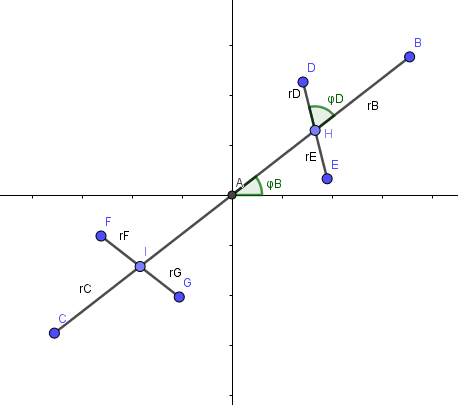
\includegraphics[width=0.75\linewidth]{schema2}}
\caption{Schéma du modèle, réalisé avec le logiciel GeoGebra}
\end{figure}

Cas particulier du modèle v2

%Paramètres fixes: 
%rayons: $r_B$, $r_C$, $r_D$, $r_E$, $r_F$, $r_G$
% 
%"rayons" de points intermédiaires : $\alpha_H$, $\alpha_I$. 
%
%Si $\alpha_H=1$, $H=B$, $\alpha_H=2$, $H$ est le milieu du segment $[BC]$, si $\alpha_H \rightarrow \infty$, $B=A$.
%
%
%paramètres input: 
%position initiale: angle: $\phi_B$, $\phi_D$, $\phi_F$
%($+ \pi$ pour les points symétriques).
%
%vitesse des moteurs: $v_1$, $v_2$, $v_3$ (nombre de tours par seconde) + sens de rotation
%
%intensité lumineuse
%
%
%On prend le point $A$ comme origine du repère.
%
%Position des points en fonction du temps (et des positions initiales):
%
%$A(x_A,y_A) = (0,0)$
%
%$B(x_B,y_B) = (r_B \cos(2 \pi v_1 t + \phi_B),r_B \sin(2 \pi v_1 t + \phi_B))$
%
%à $t=0$, $B = (r_B \cos(\phi_B), r_B \sin(\phi_B))$
%
%$C(x_C,y_C) = (r_C \cos(2 \pi v_1 t + \phi_B + \pi),r_C \sin(2 \pi v_1 t + \phi_B + \pi))$
%
%$H(x_H,y_H) = ( \frac{r_B}{\alpha_H} \cos(2 \pi v_1 t + \phi_B),\frac{r_B}{\alpha_H} \sin(2 \pi v_1 t + \phi_B))$
%
%De même,
%$I(x_I,y_I) = ( \frac{r_C}{\alpha_I} \cos(2 \pi v_1 t + \phi_B + \pi), \frac{r_C}{\alpha_I} \sin(2 \pi v_1 t + \phi_B + \pi))$
%
%Pour déterminer la position des points $D,E,F,G$, on utilise les points intermédiaires ($H$ et $I$), (utilise le changement de repère  orthonormale centrée en H et de vecteurs directeurs un  de même direction que $\overrightarrow{AH}$, l'autre orthogonal, dans lequel $\overrightarrow{HD} =  rD( \cos(2 \pi v_2 t + \phi_D), \sin(2 \pi v_2 t + \phi_D))$)
%
%%$ D(t) = (x_D(t),y_D(t)) = (\frac{r_B}{\alpha_H} \cos(2 \pi v_1 t + \phi_B) + r_D \cos(2 \pi (v_2 + v _1)t + (\phi_D + \phi_B)), \frac{r_B}{\alpha_H} \sin(2 \pi v_1 t + \phi_B ) + r_D \sin(2 \pi (v_2 +v_1)t +  (\phi_D + \phi_B))  )$
%
%$
%D(t)=
%\begin{pmatrix}
%x_D(t) \\ 
%y_D(t)
%\end{pmatrix}
%=
%\begin{pmatrix}
%\frac{r_B}{\alpha_H} \cos(2 \pi v_1 t + \phi_B) + r_D \cos(2 \pi (v_2 + v _1)t + (\phi_D + \phi_B) \\ 
%\frac{r_B}{\alpha_H} \sin(2 \pi v_1 t + \phi_B ) + r_D \sin(2 \pi (v_2 +v_1)t +  (\phi_D + \phi_B))  
%\end{pmatrix}
%$
%
%%$ \overrightarrow{HD} = (r_D \cos(2 \pi v_2 t + \phi_D),r_D \sin(2 \pi v_2 t + \phi_D))$
%%
%%
%%Donc  $ \overrightarrow{AD} = \overrightarrow{AH} + \overrightarrow{HD} = (\frac{r_B}{\alpha_H} \cos(2 \pi v_1 t + \phi_B) + r_D \cos(2 \pi v_2 t + \phi_D), \frac{r_B}{\alpha_H} \sin(2 \pi v_1 t + \phi_B)) + r_D \sin(2 \pi v_2 t + \phi_D)  )$
%%
%%Donc $ D = (x_D,y_D) = (\frac{r_B}{\alpha_H} \cos(2 \pi v_1 t + \phi_B) + r_D \cos(2 \pi v_2 t + \phi_D), \frac{r_B}{\alpha_H} \sin(2 \pi v_1 t + \phi_B)) + r_D \sin(2 \pi v_2 t + \phi_D)  )$
%
%
%Vitesse de $D$ au temps $t$:
%
%%$ D'(t) = (x'_D(t),y'_D(t)) = (-\frac{r_B}{\alpha_H} 2 \pi v_1 \sin(2 \pi v_1 t + \phi_B) - r_D 2 \pi (v_2 + v _1) \sin(2 \pi (v_2 + v _1)t + (\phi_D + \phi_B)), \frac{r_B}{\alpha_H} 2 \pi  v_1 \cos(2 \pi v_1 t + \phi_B ) + r_D  2 \pi (v_2 + v _1) \cos(2 \pi (v_2 +v_1)t +  (\phi_D + \phi_B))  )$
%
%
%$
%D'(t)=
%\begin{pmatrix}
%x'_D(t) \\ 
%y'_D(t)
%\end{pmatrix}
%=
%\begin{pmatrix}
%-\frac{r_B}{\alpha_H} 2 \pi v_1 \sin(2 \pi v_1 t + \phi_B) - r_D 2 \pi (v_2 + v _1) \sin(2 \pi (v_2 + v _1)t + (\phi_D + \phi_B)) \\ 
%\frac{r_B}{\alpha_H} 2 \pi  v_1 \cos(2 \pi v_1 t + \phi_B ) + r_D  2 \pi (v_2 + v _1) \cos(2 \pi (v_2 +v_1)t +  (\phi_D + \phi_B))  
%\end{pmatrix}
%$
%
%
%Accélération de $D$ au temps $t$:
%
%$ D''(t) = (x''_D(t),y''_D(t)) = (-\frac{r_B}{\alpha_H} (2 \pi v_1)^2 \cos(2 \pi v_1 t + \phi_B) - r_D  (2 \pi (v_2 + v _1))^2 \cos(2 \pi (v_2 + v _1)t + (\phi_D + \phi_B)), - \frac{r_B}{\alpha_H} (2 \pi  v_1)^2 \sin(2 \pi v_1 t + \phi_B ) - r_D  (2 \pi (v_2 + v _1))^2 \sin(2 \pi (v_2 +v_1)t +  (\phi_D + \phi_B))  )$
%
%
%$
%D''(t)=
%\begin{pmatrix}
%x''_D(t) \\ 
%y''_D(t)
%\end{pmatrix}
%=
%\begin{pmatrix}
%-\frac{r_B}{\alpha_H} (2 \pi v_1)^2 \cos(2 \pi v_1 t + \phi_B) - r_D  (2 \pi (v_2 + v _1))^2 \cos(2 \pi (v_2 + v _1)t + (\phi_D + \phi_B)) \\ 
%- \frac{r_B}{\alpha_H} (2 \pi  v_1)^2 \sin(2 \pi v_1 t + \phi_B ) - r_D  (2 \pi (v_2 + v _1))^2 \sin(2 \pi (v_2 +v_1)t +  (\phi_D + \phi_B))  )  
%\end{pmatrix}
%$
%
%
%
%Remarque: soit $\alpha \in \R$, (pour tout $v_1,v_2,t$)
%
%$B(\alpha v_1,t) = B(v_1,\alpha t)$,
%
%$D(\alpha v_1,\alpha v_2,t) = D(v_1,v_2,\alpha t)$
%
%Donc multiplier les 3 vitesses par un facteur identique ne changera pas la figure totale obtenue (l'image de tout les temps): il existe un temps (et on sait lequel), auquel le point sera au même endroit que pour l'autre vitesse. Une différence peut intervenir si l'on considère la persistance rétinienne.






\subsection{Stationnaire (v2)}

Nouveau modèle, nouveau schéma, nouvelles équations.

\begin{figure}[H] 
\center{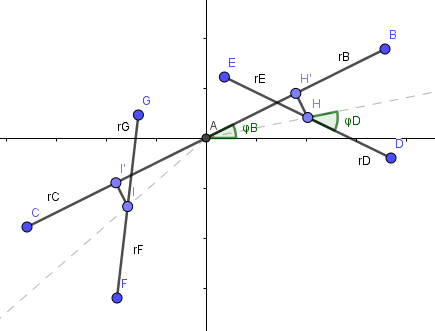
\includegraphics[width=0.75\linewidth]{schema3}}
\caption{Schéma du modèle v2, réalisé avec le logiciel GeoGebra}
\end{figure}


Paramètres fixes: 
rayons: $r_B$, $r_C$, $r_D$, $r_E$, $r_F$, $r_G$, $r_H$, $r_I$,
 
angle: $\alpha_H$,  $\alpha_I$ (supposés positifs)


paramètres input: 
position initiale (angle): $\phi_B$, $\phi_D$, $\phi_F$
($+ \pi$ pour les points symétriques).

vitesse des moteurs: $v_1$, $v_2$, $v_3$ (nombre de tours par seconde) + sens de rotation

intensité lumineuse


On prend le point $A$ comme origine du repère.

Position des points en fonction du temps (et des positions initiales):

$A(x_A,y_A) = (0,0)$

$B(x_B,y_B) = (r_B \cos(2 \pi v_1 t + \phi_B),r_B \sin(2 \pi v_1 t + \phi_B))$

à $t=0$, $B = (r_B \cos(\phi_B), r_B \sin(\phi_B))$

$C(x_C,y_C) = (r_C \cos(2 \pi v_1 t + \phi_B + \pi),r_B \sin(2 \pi v_1 t + \phi_B + \pi))$

$H(x_H,y_H) = ( r_H \cos(2 \pi v_1 t + \phi_B - \alpha_H), r_H \sin(2 \pi v_1 t + \phi_B - \alpha_H))$

De même,
$I(x_I,y_I) = ( r_I \cos(2 \pi v_1 t + \phi_B + \pi + \alpha_I),  r_I \sin(2 \pi v_1 t + \phi_B + \pi + \alpha_I))$

Noter la différence de signe entre $\alpha_H$ et $\alpha_I$.

Pour déterminer la position des points $D,E,F,G$, on utilise les points intermédiaires $H$ et $I$, et une formule de changement de base, ou de la trigo.

%(utilise le changement de repère  orthonormale centrée en H et de vecteurs directeurs un  de même direction que $\overrightarrow{AH}$, l'autre orthogonal, dans lequel $\overrightarrow{HD} =  rD( \cos(2 \pi v_2 t + \phi_D), \sin(2 \pi v_2 t + \phi_D))$)

%$ D(t) = (x_D(t),y_D(t)) = (\frac{r_B}{\alpha_H} \cos(2 \pi v_1 t + \phi_B) + r_D \cos(2 \pi (v_2 + v _1)t + (\phi_D + \phi_B)), \frac{r_B}{\alpha_H} \sin(2 \pi v_1 t + \phi_B ) + r_D \sin(2 \pi (v_2 +v_1)t +  (\phi_D + \phi_B))  )$

$
D(t)=
\begin{pmatrix}
x_D(t) \\ 
y_D(t)
\end{pmatrix}
=
\begin{pmatrix}
r_H \cos(2 \pi v_1 t + \phi_B- \alpha_H )  + r_D \cos(2 \pi (v_2 + v _1)t + (\phi_D + \phi_B - \alpha_H) \\ 
r_H \sin(2 \pi v_1 t + \phi_B - \alpha_H) + r_D \sin(2 \pi (v_2 +v_1)t +  (\phi_D + \phi_B - \alpha_H))  
\end{pmatrix}
$


Vitesse de $D$ au temps $t$:

$
D'(t)=
\begin{pmatrix}
x'_D(t) \\ 
y'_D(t)
\end{pmatrix}
=
\begin{pmatrix}
- r_H  2 \pi v_1 \sin(2 \pi v_1 t + \phi_B - \alpha_H) - r_D 2 \pi (v_2 + v _1) \sin(2 \pi (v_2 + v _1)t + (\phi_D + \phi_B - \alpha_H)) \\ 
  r_H  2 \pi  v_1 \cos(2 \pi v_1 t + \phi_B - \alpha_H) + r_D  2 \pi (v_2 + v _1) \cos(2 \pi (v_2 +v_1)t +  (\phi_D + \phi_B - \alpha_H))  
\end{pmatrix}
$


Accélération de $D$ au temps $t$:

$
D''(t)=
\begin{pmatrix}
x''_D(t) \\ 
y''_D(t)
\end{pmatrix}
=
\begin{pmatrix}
-r_H (2 \pi v_1)^2 \cos(2 \pi v_1 t + \phi_B - \alpha_H) - r_D  (2 \pi (v_2 + v _1))^2 \cos(2 \pi (v_2 + v _1)t + (\phi_D + \phi_B- \alpha_H)) \\ 
- r_H (2 \pi  v_1)^2 \sin(2 \pi v_1 t + \phi_B - \alpha_H) - r_D  (2 \pi (v_2 + v _1))^2 \sin(2 \pi (v_2 +v_1)t +  (\phi_D + \phi_B - \alpha_H))  )  
\end{pmatrix}
$



Remarque: soit $\alpha \in \R$, (pour tout $v_1,v_2,t$)

$B(\alpha v_1,t) = B(v_1,\alpha t)$,

$D(\alpha v_1,\alpha v_2,t) = D(v_1,v_2,\alpha t)$

Donc multiplier les 3 vitesses par un facteur identique ne changera pas la figure totale obtenue (l'image de tout les temps): il existe un temps (et on sait lequel), auquel le point sera au même endroit que pour l'autre vitesse. Une différence peut intervenir si l'on considère la persistance rétinienne.




\subsection{Persistance rétinienne}

Il semblerait que l’oeil garde une image rémanente pendant 1/25 seconde sur la rétine.

Dans le modèle, cela reviendrait non pas à avoir en sortie à l'instant $t$ la position des lumières à cet instant, mais l'ensemble des positions des lumières occupées durant les 1/25 secondes précédentes. Remarque, plus les vitesses des moteurs (donc de déplacement des lumières) sont importantes, plus les lumières parcourent de distance pendant ces 1/25 secondes, et donc plus les figurent ont une grande "longueur".


\subsection{Transitoire}

piste ? Relier la tension d'entrée du moteur $u$ à la sortie: vitesse angulaire $\omega$. L'idée serait que quand on tourne le bouton, on fait varier la tension du moteur et donc sa vitesse (prendre en compte l'inertie). On pourrait donc chercher des fonctions du temps comme contrôle du système (la position du bouton de contrôle du moteur).

Une source pour les équations sur un moteur...
\url{https://www.wikimeca.org/index.php/Moteur_\%C3\%A0_courant_continu}

Les paramètres:

Partie électrique:
\begin{itemize}
\item $R$ est la résistance électrique interne du moteur (Ohm)
\item  $K_e$ est la constante de force électromotrice
\end{itemize}


Partie mécanique
\begin{itemize}
\item $J$  rotor vu comme un volant d'inertie $J$  
\item $K_c$ est la constante de couple  
\item $f$ est le coefficient de frottement visqueux.
\end{itemize}


Les deux quantités qui interviennent dans l'équation différentielle simplifiée (pas d'inductance):

$A =  \frac{K_c}{(R*f+K_c*K_e)}$

$C = \frac{J*R}{(R*f+K_c*K_e)}$


On suppose connu les valeurs de ces paramètres pour les trois moteur de l'installation (soit mesurés physiquement, soit c'est donné par le fabriquant, au pire par calibration?)

La dynamique du moteur simplifiée est décrite par:

point de vue fonction de transfert:
$ H(p) = \frac{\Omega(p)}{U(p)} = \frac{A}{C*p+1}$

point de vue EDO:
$C * \omega'(t) + \omega(t) = A*u(t)$


solution, en imposant $y(0) = \omega(0) = 0$: $\omega(t) := y(t) = e^{-\frac{t}{C}} * \int_0^t \frac{A}{C} u(x) e^{\frac{x}{C}} dx $


On suppose les trois moteurs "indépendants", ils ont chacun leurs paramètres (électriques et mécaniques) mais fonctionnent selon les mêmes équations.
Dans le régime stationnaire, on supposait la vitesse des moteurs constante au cours du temps (égale  respectivement à $v_1$, $v_2$ et $v_3$). Désormais, cette vitesse $\omega_1, \omega_2, \omega_3$ peut varier au cours du temps, en particulier, on suppose qu'elle est nulle initialement, puis qu'on applique une tension au moteur. Les équations de la dynamique dans le cadre stationnaire sont ainsi conservées, et seule la vitesse $v_i$ est remplacée par $\omega_i$, donc l'angle à l'instant $t$ n'est plus $v_1 *t$ mais $ \int_0^t v_1(x)dx$ (condition initiale nulle).

Remarque: Si on applique une tension constante $U$, la vitesse de rotation en sortie tend vers $U*A$. On peut déduire de cette dernière égalité la valeur de la tension à appliquer au moteur pour obtenir la vitesse de rotation désirée.




\section{Étude mathématique...}
... pour le modèle stationnaire

Courbe paramétrée pour la dynamique de chacun de points. On se concentre d'abord sur la courbe paramétrée produite par un point, on pourra ensuite éventuellement s'intéresser à la figure produite par tous les points (union des courbes paramétrées).

Étude des points singulier: condition nécessaire pour en avoir.

Étude de la périodicité: condition suffisante si il existe $m,n \in \N$ tels que $ \frac{m}{v_1}= \frac{n}{v_1+ v_2}$. 

Étude de de la monotonie de chaque composantes ($x$ et $y$) 

Points doubles: $t_1$ et $t_2$ tels que: $x(t_1)=x(t_2)$ et $y(t_1) = y(t_2)$.



\section{Mesures}

On illustre les mesures sur une trajectoire obtenue avec les paramètres suivants:

angles initiaux: $angleIniB = 0$ , $angleIniD = 1$ , $angleIniF = 2$

et les vitesses:
$v_1 = 1.8$ , $v_2= -2.66$ , $v_3 = 3.14$  

Tfinal = 10, deltaT = 0.0005.

Les trajectoires des points sont tracées sur la figure \ref{trajectoire_exemple_mesure} .

\begin{figure}[H] 
\center{\includegraphics[width=0.75\linewidth]{figure_trajectoires_exemple_mesures}}
\caption{Trajectoires pour illustrer les mesures}
\label{trajectoire_exemple_mesure}
\end{figure}

\bigbreak

\textbf{Densité}

La trajectoire remplit l'espace ?
Densité d'occupation des points de la trajectoire sur une grille: densité pour la trajectoire d'un point et pour les différents points. Paramètre: la pas de la subdivision de la grille


\textbf{Points singuliers:} leur nombre et les indices (temps) auxquels ils apparaissent. Paramètre: seuil sur la dérivée

Dans l'exemple, seules les trajectoires des points D et E présentent des points singuliers (figure \ref{mesure_singulierD})

\begin{figure}[H] 
\center{\includegraphics[width=0.55\linewidth]{singulierD}}
\caption{Les 27 points singuliers de la trajectoire du point D}
\label{mesure_singulierD}
\end{figure}




\textbf{Boucle / temps de retour:} nombre, indice (temps) du point concerné, et la durée (nombre de pas te temps) de la boucle, aussi la distribution des angle des points boucles.

Dans l'exemple, les trajectoires des points D et E ainsi que celles de F et G présentent des points de retour (figures \cref{mesure_retourD,mesure_retourF})

\begin{figure}[H] 
\center{\includegraphics[width=0.55\linewidth]{retourD}}
\caption{Points de retour pour la trajectoire D}
\label{mesure_retourD}
\end{figure}

\begin{figure}[H] 
\center{\includegraphics[width=0.55\linewidth]{retourF}}
\caption{Points de retour pour la trajectoire F}
\label{mesure_retourF}
\end{figure}


Sur la figure \ref{mesure_retourD_color}, les couleurs correspondent à des points ayant des temps de retour identiques.

\begin{figure}[H] 
\center{\includegraphics[width=0.55\linewidth]{retourD_ordered_color}}
\caption{Temps de retour pour la trajectoire D}
\label{mesure_retourD_color}
\end{figure}




\textbf{Courbure de la trajectoire:} en chaque point la courbure. Regarder la moyenne ou d'autres information statistique sur la distribution des rayons de courbure. %Pas de paramètre. On peut aussi repérer des morceaux de trajectoires qui ressemblent à une droite (courbure nulle: seuil) ou à un cercle (courbure constante).
%concavité/ convexité locale?: rayon de courbure: les distribution des rayons de courbure sur la trajectoire: diversité ou uniforme ?


Les figures \cref{mesure_ourbureB,mesure_ourbureD,mesure_ourbureF} représentent respectivement les courbures pour les points des trajectoire des points B, D et F. La trajectoire de B est un cercle, le rayon de courbure est donc constant.


\begin{figure}[H] 
\center{\includegraphics[width=0.55\linewidth]{courbureB}}
\caption{Rayon de courbure pour la trajectoire B}
\label{mesure_ourbureB}
\end{figure}


\begin{figure}[H] 
\center{\includegraphics[width=0.55\linewidth]{courbureD}}
\caption{Rayon de courbure pour la trajectoire D}
\label{mesure_ourbureD}
\end{figure}


\begin{figure}[H] 
\center{\includegraphics[width=0.55\linewidth]{courbureF}}
\caption{Rayon de courbure pour la trajectoire F}
\label{mesure_ourbureF}
\end{figure}





\textbf{Indice de Moran:} sur l'agrégation spatiale.


\textbf{Autres idées:} (pas implémentées)

Nombre de composantes connexes dans l'espace (Julien ?, JTS lib scala pour les trucs de géométrie)
%https://locationtech.github.io/jts/javadoc/org/locationtech/jts/geom/Geometry.html

La courbe est elle fermée (périodicité)?



\subsection{Les mesures retenues}
Pour une trajectoire avec des lumières allumées/ éteintes:

\begin{itemize}
\item nombre de points singuliers
\item nombre de point de retour
\item densité totale (+ celle de D/F)
\item indice Moran total (+ D/F)
\item courbure moyenne: toutes les trajectoires
\end{itemize}





%%%%%%%%%%%%%%%%%%           END      %%%%%%%%%%%%%%%%%%%%%%%%%%%%%%%%%

 
\end{document}

